\subsection{Physical Setup}
\label{sec:PhysicalSetup}


The setup must model a room with luminaires on its ceiling. Each luminaire has a controller that keeps the light below it above some standard level of illuminance. For this project it was pre-established that the room contained three luminaires.

For the physical setup a wooden box was used. This was preferred to a cardboard box because of the increased sturdiness. Since the controllers (Arduinos) are too big to be included inside the luminaires in our model they were put on the outside of the box,  and all the wiring is done outside the box using a breadboard (see \autoref{fig:setup_box_closed}). Both the breadboard and the Arduinos are screwed to the box preventing them to move, which could easily disconnect the jumpers. Tight holes were made to pass the wires needed to light the LED and read the sensor, while preventing light from entering the box (see \autoref{fig:setup_arduino_connections}).

\begin{figure}[h]
    \centering
    \begin{subfigure}[t]{0.49\textwidth}
        \centering
        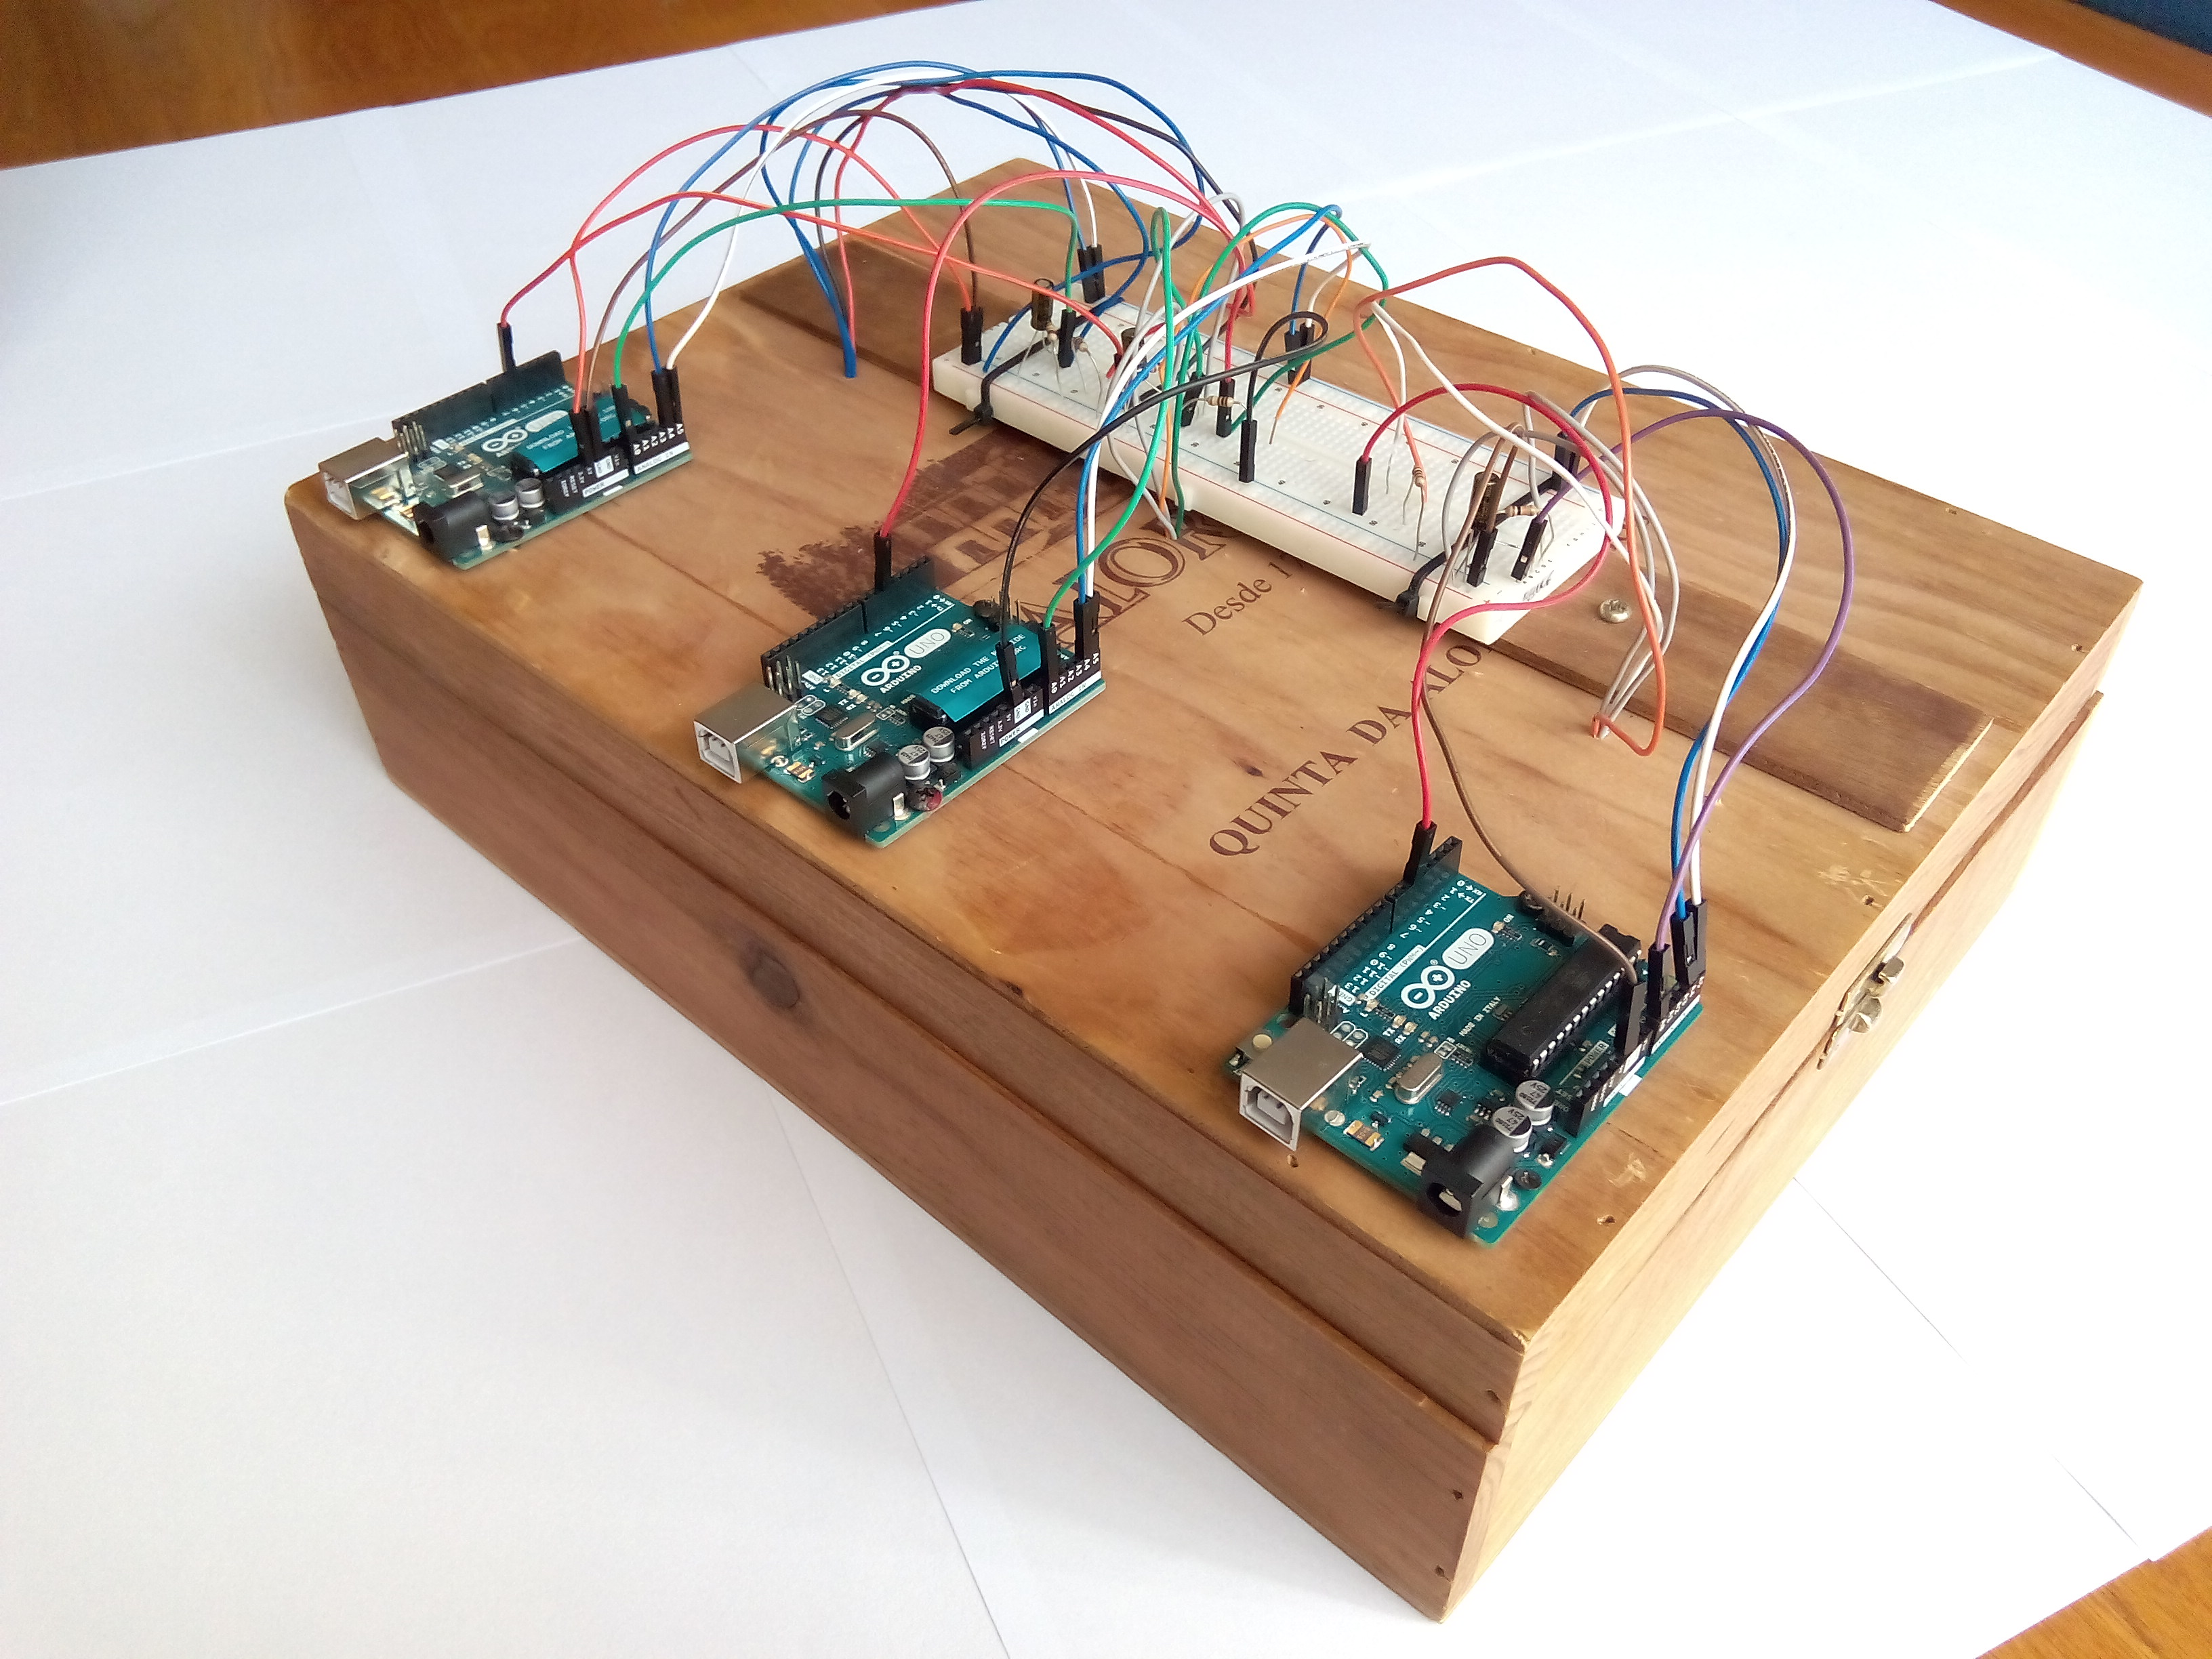
\includegraphics[width=\textwidth]{img/setup_box_closed}
        \caption{Arduinos and breadboard on top of the box}
        \label{fig:setup_box_closed}
    \end{subfigure}
    \begin{subfigure}[t]{0.49\textwidth}
        \centering
        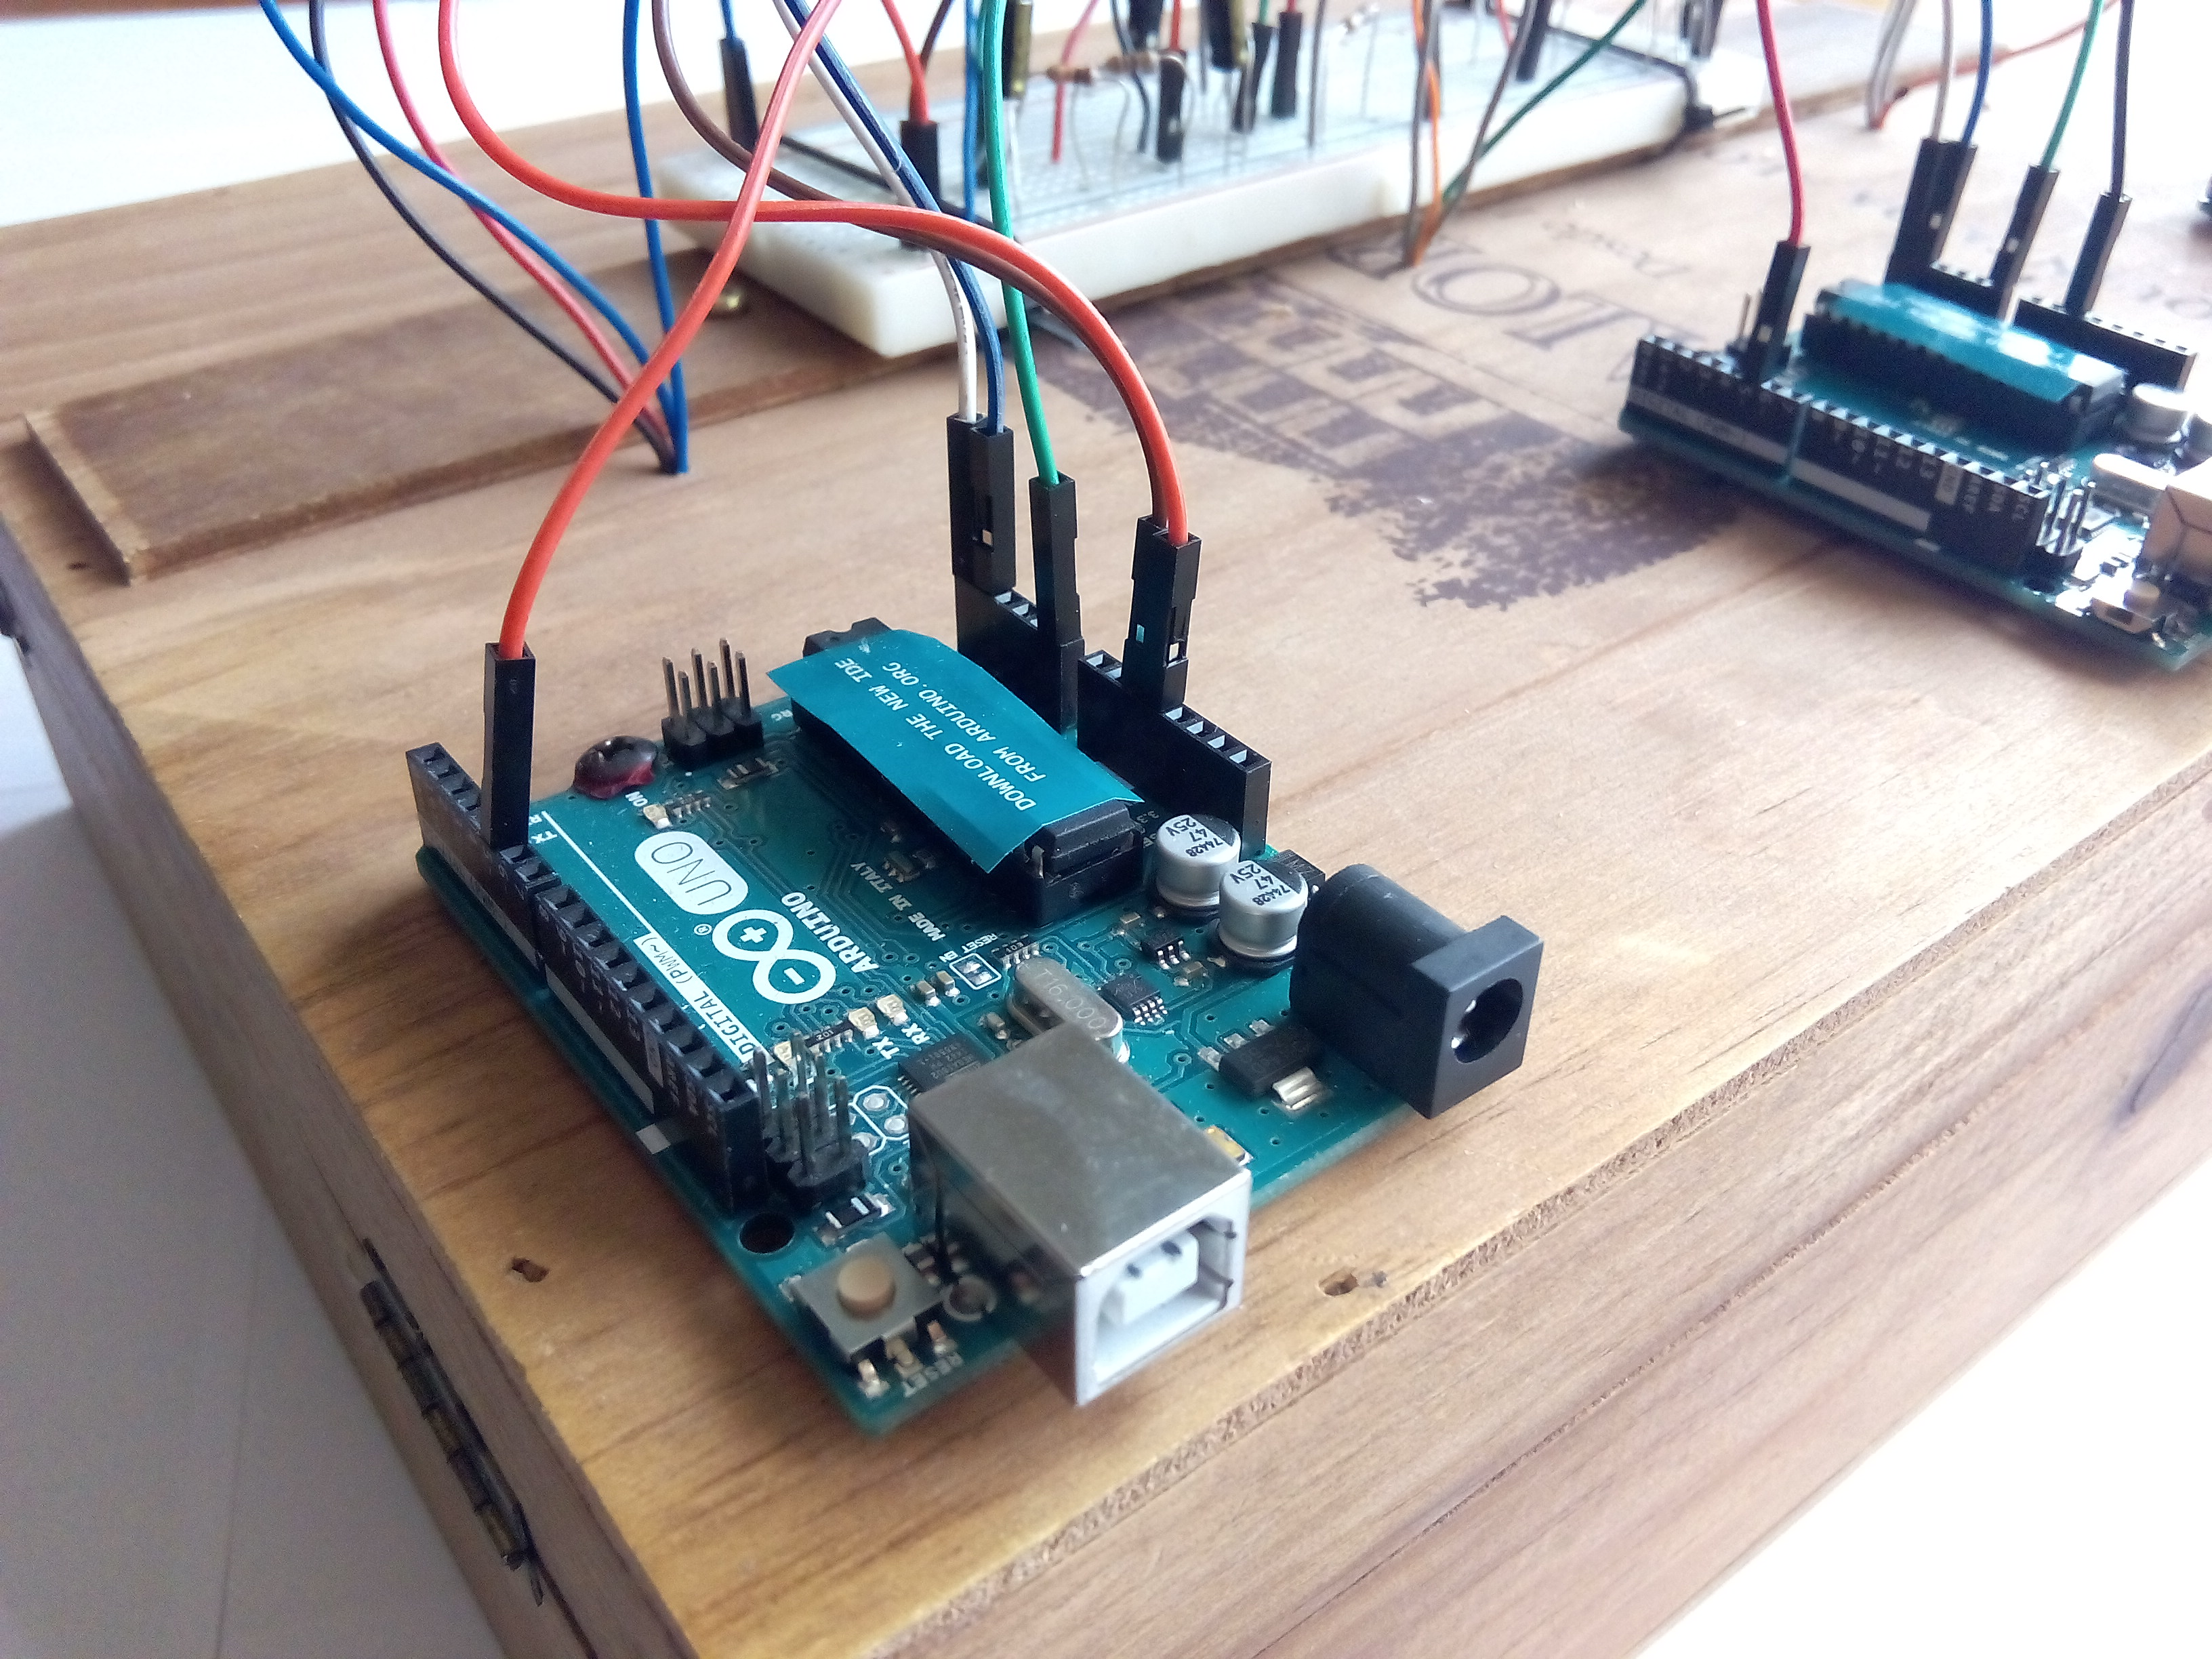
\includegraphics[width=\textwidth]{img/setup_arduino_connections.jpg}
        \caption{Detail showing the connections on the Arduino and one hole in the box}
        \label{fig:setup_arduino_connections}
    \end{subfigure}
    \caption{The outside of the box}
    \label{fig:setup_box_outside}
\end{figure}


On the inside of the box only the luminaires are present. Each luminaire is assumed to include both a LED light and a light sensor (LDR). The LED and the LDR are separated by a piece of cardboard so that the light from the LED does not directly affect the LDR reading (\autoref{fig:setup_box_open}). Only reflected light should be read. In order to increase the light reflection inside the box --- so that the LDR senses more light --- a white sheet of paper was placed on the bottom of the box (see \autoref{fig:setup_LDR_LED}).

\begin{figure}[h]
    \centering
    \begin{subfigure}[t]{0.49\textwidth}
        \centering
        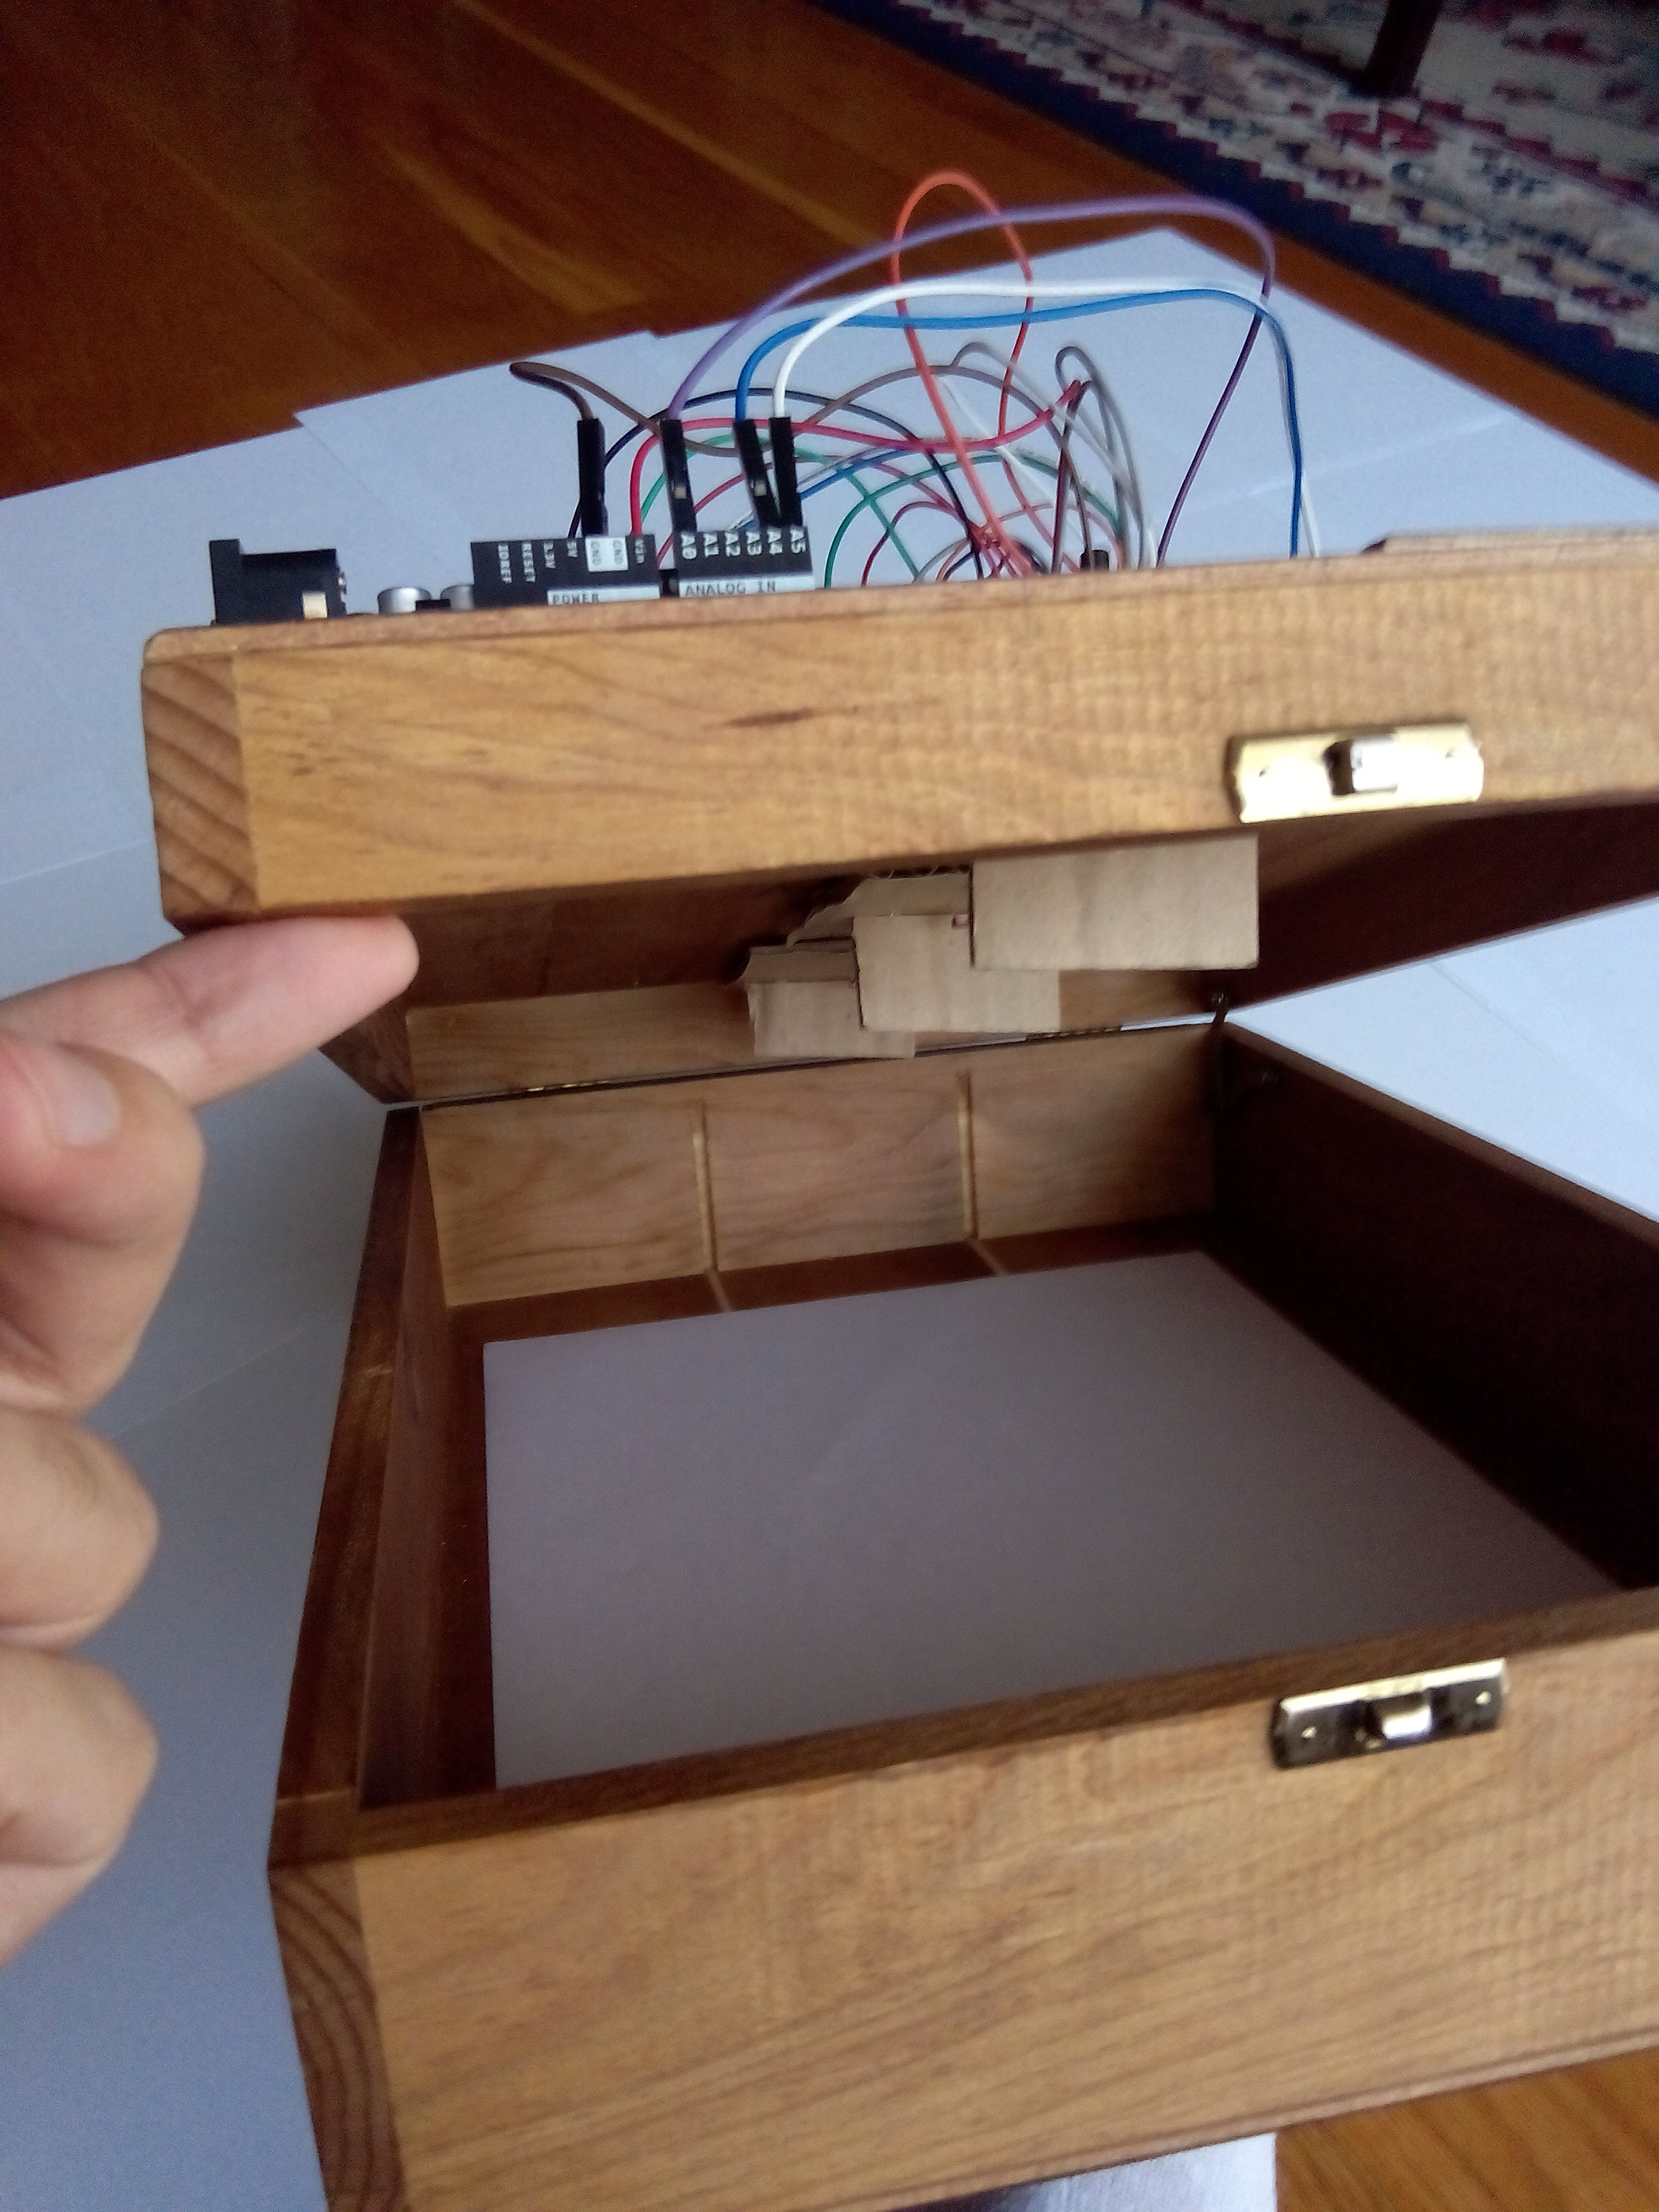
\includegraphics[width=\textwidth]{img/setup_box_open}
        \caption{Luminaires on the ceiling and white sheet on the floor}
        \label{fig:setup_box_open}
    \end{subfigure}
    \begin{subfigure}[t]{0.49\textwidth}
        \centering
        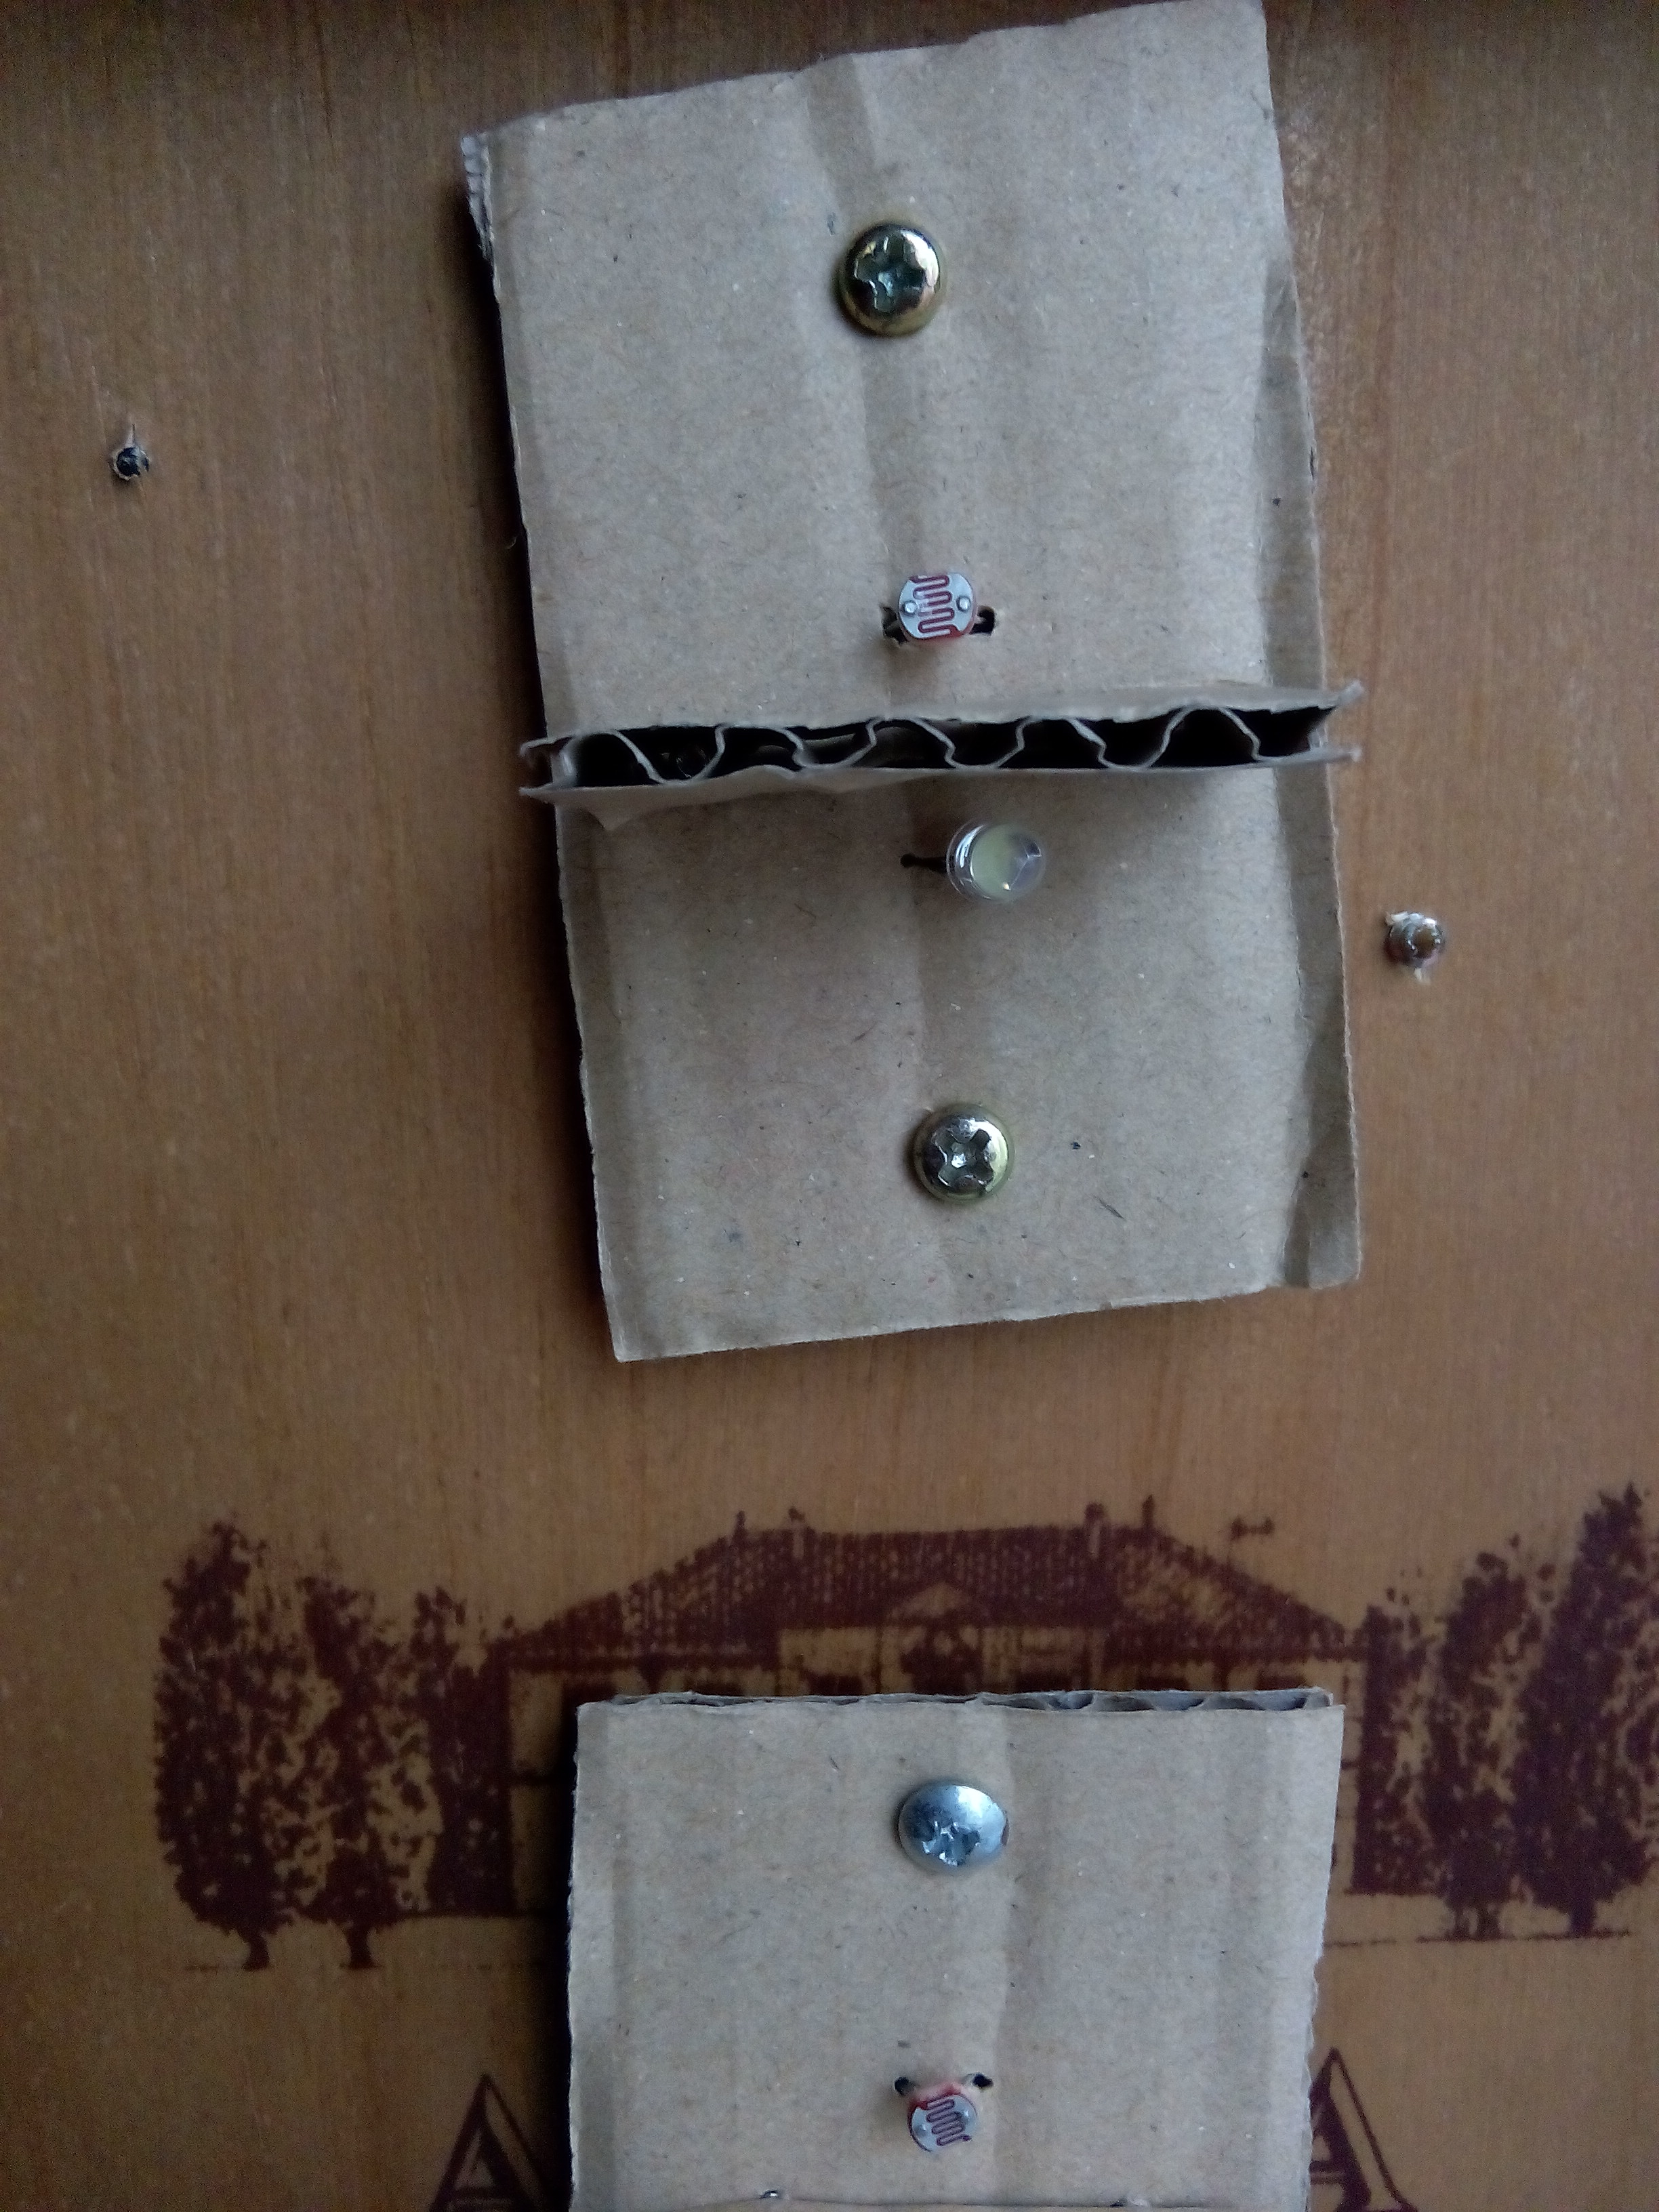
\includegraphics[width=\textwidth]{img/setup_LDR_LED}
        \caption{Detail of a luminaire. The LDR on top, LED on bottom and cardboard in between}
        \label{fig:setup_LDR_LED}
    \end{subfigure}
    \caption{The inside of the box}
    \label{fig:setup_box_inside}
\end{figure}

The assignment requires that the model has a window. The used box has hinges and the top of the box can be opened (see \autoref{fig:setup_LDR_LED}). Therefore this was used as an window. The top should only be opened in small angles so that we can consider (by approximation) that the LDR is still facing the ground and that the light of the LED is mostly reflected back at the LDR.

% about the circuits

The emitter-detector circuit for each luminaire is shown in \autoref{fig:setup_circuits}. The emitter is made of an LED in series with a current limiting resistor (\autoref{fig:setup_LED_circuit}). The typical forward voltage of the used LED is \SI{3.0}{\volt} and its maximum forward current is \SI{20}{\milli\ampere}. Since the Arduino is powered with \SI{5}{\volt} the voltage on pin \texttt{D5} is at most \SI{5}{\volt}. Therefore, using a \SI{100}{\ohm} resistor makes the LED be at its maximum power when the duty cycle on pin \texttt{D5} is 1. For the light detector circuit a voltage divider is used, consisting of a normal resistor and a photoresistor. A capacitor is also included in parallel with the resistor to act as a low-pass filter to eliminate noise from the readings. An analysis of the characteristic of the LDR is made in \ref{subsubsec:LDR_model}.

\begin{figure}[h]
    \centering
    \begin{subfigure}[t]{0.49\textwidth}
        \centering
        \begin{circuitikz} \draw
            (0,0) node[sground] {}
            to[resistor, l_=\mbox{$R_1 = \SI{100}{\ohm}$}] (0,2);
            \draw (0,4) to[empty led, l=$D_1$] (0,2) ;
			\draw (0,4) to[short, -o] (-1.5,4)
            node[left]{\texttt{D5}}
            ;
        \end{circuitikz}
        \caption{The LED circuit. Pin \texttt{D5} controls the power on the LED using PWM.}
        \label{fig:setup_LED_circuit}
    \end{subfigure}
    \begin{subfigure}[t]{0.49\textwidth}
        \centering
        \begin{circuitikz} \draw
            (0,0) node[sground] {}
            to[resistor, l=\mbox{$R_3 = \SI{10}{\kilo\ohm}$}] (0,2)
            to[photoresistor, l=$R_2$] (0,4)
            to[short, -o] (0,4.5)
            node[right]{$V_S = 5 V$}

            (1,0) node[sground] {}
            to[polar capacitor, l_=\mbox{$C_1 = \SI{1}{\micro\farad}$}] (1,2)
            (0,2) -- (1,2)

            (1,2) to[short, -o] ++(2,0)
            node[right]{\texttt{A0}}
            ;
        \end{circuitikz}
        \caption{The light detector. An LDR is used and readings are done on pin \texttt{A0}.}
        \label{fig:setup_LDR_circuit}
    \end{subfigure}
    \caption{Emitter-detector circuitry of each luminaire}
    \label{fig:setup_circuits}
\end{figure}

A I\textsuperscript{2}C/TWI bus is used to implement the communications between the controllers of each luminaire. The physical implementation of this bus is attained by connecting the \texttt{A4} pin of all the Arduinos as well as the \texttt{A5} pins --- SDA and SCL respectively.
